\scanpage{91}

\deleted{\unsure{The formula}} Finally, if $\xi=(\xi_i)$ is any sequence of \deleted{positive} real numbers, set $x_n=(\unsure{\xi_1|\xi'_1}\mathord{-}\xi_n,0,\mathord{-}0)$, then $N(x_n)$ \deleted{has a limit \unsure{when} \illegible{1} of $n$}, \inserted{increases with $n$, and} we set $N(\xi)=N((\xi_i))=\lim_n N(x_n)$, a finite or infinite number. $\geq0$

\deleted{\unsure{Thus|Then}} The formula (25) is a special case of the theorem, for $N$ \deleted{\unsure{enjoys the properties}}\inserted{satisfies the} conditions envisaged for $f$ in this statement. The formula (26) follows from it by passage to the limit.

{\reversemarginpar\margin{\uline{Theorem 3}}}\uline{Second convexity theorem in Hilbert spaces}

{\reversemarginpar\margin{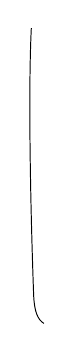
\begin{tikzpicture}[x=1cm,y=1cm]\draw[line width=.35pt] (0,0) .. controls (-.04,-.8) and (-.01,-2.3) .. (.03,-3.4) .. controls (.04,-3.6) and (.08,-3.7) .. (.16,-3.75);\end{tikzpicture}}}
Le\deleted{\unsure{t}}\inserted{\unsure{t|t}} $E,F,\unsure{C|G}$ be three Hilbert spaces, let $u$ be a \deleted{continuous}\inserted{compact} linear map from $E$ to $F$, \deleted{$E$} $v$ a \deleted{continuous}\inserted{compact} linear map from $F$ to $\unsure{C|G}$, \deleted{let $\unsure{u|n}$ be a positive integer} finally let $f(s_1,\mathord{-}s_n)$ be a continuous \inserted{symmetric and increasing} function of $n$ arguments $s_i\geq0$, such that \deleted{the function} $f(e^{t_1},\mathord{-},e^{t_n})$ is a convex function of $(t_i)\in R^n$. Then we have

\[
\begin{array}{@{}l@{\qquad}l@{}}
(29)&\displaystyle f(\rho_1(uv),\mathord{-}\rho_n(uv))\leq f(\rho_1(u)\rho_1(v),\mathord{\cdot}\,\mathord{-},\rho_n(u)\rho_n(v)\unsure{,})
\end{array}
\]

Indeed, it suffices to \deleted{combine}\inserted{\unsure{apply it|apply}} the \deleted{lemma}\inserted{theorem 1} \deleted{fundamental, \unsure{corollary} 1, \unsure{condition}} to the two sequences $(\rho_i(uv))_{i\leq n}$ and $(\rho_i(u)\rho_i(v))_{i=n}$. The conditions \inserted{in hypothesis b number 2°) of theorem 1.} of the \deleted{corollary 1 of this lemma} are satisfied, \deleted{\unsure{indeed}} by virtue of number \unsure{?|7}, proposition 2, corollary 3. \deleted{(\unsure{indeed} \illegible{1})}.

\uline{Corollary 1} Let $u$ and $v$ be \deleted{as} in theorem 3, let $f(r)$ be a continuous increasing function of $r\geq0$ such that $f(e^t)$ is a convex function of $t\in R$. Then, for \deleted{every \unsure{number}} integer $n>0$, we have

{\reversemarginpar\margin{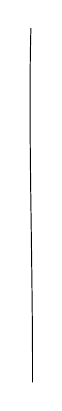
\begin{tikzpicture}[x=1cm,y=1cm]\draw[line width=.35pt] (0,0) .. controls (-.035,-1.25) and (.025,-3) .. (.02,-4.5);\end{tikzpicture}}}
{\reversemarginpar\margin{\illegible{1} $\unsure{l}$\\\deleted{\illegible{1}}\\\deleted{\illegible{1}}\\\deleted{\illegible{1}}}}
\[
\begin{array}{@{}l@{\qquad}l@{}}
(30)&\displaystyle \sum_{i=1}^n f(\rho_i(uv))\leq\sum_{i=1}^n f(\rho_i(u)\rho_i(v))
\end{array}
\]

\deleted{whence} \inserted{whence}

\[
\begin{array}{@{}l@{\qquad}l@{}}
(3\unsure{1|4})&\displaystyle \sum_{\unsure{j|i}} f(\rho_i(uv))\leq\sum_{i\unsure{\mathord{-}|=}} f(\rho_i(u)\rho_i(v))
\end{array}
\]

(the sums being extended over all indices $i$.)

\deleted{\illegible{1} $\unsure{(\rho_i(uv))|(\rho_i(vu))}$ \unsure{associated} \illegible{2} \unsure{of the sequences} $(\rho_i(u))$}

\deleted{$(\rho_i(v))$ associated with $u$ resp. $v$, \unsure{the|the} $=$s \unsure{upper bound|upper bounds} \deleted{\unsure{for every}} as the one that would hold if we had $\unsure{\cdot}uv)=\rho_i(u)\rho_i(v)$, thus if $u$ and $v$ were multiplication \unsure{p}erators on $l^{\unsure{?|2}}$ by the \unsure{tes} $(\rho_i(u))$ resp.\textsuperscript{t} $(\rho_i(v))$. \deleted{\unsure{By specializing}} \inserted{\uline{But} \unsure{foresee|why|could} also.} \deleted{\unsure{the latter, it}} give a corollary \deleted{which} analogous \deleted{\uline{\unsure{Theorem 4}} \unsure{Let}} to corollary 4 of theorem 1, but \unsure{of it|we} leave \unsure{the statement} \unsure{to the} reader.}

\deleted{In inequality (39), \unsure{let us take} $p$ \unsure{fixed|finite} and \unsure{very} \illegible{1} $q$ towards $0$, \unsure{whence|$u$} given by (30) \illegible{1} and \unsure{we obtain} in the \unsure{limit}}

{\reversemarginpar\margin{92}}
